\chapter{Il modello lineare nei parametri}

\textbf{Problema di riferimento:} come il prezzo influenza il consumo di
gas? Si hanno a disposizione le informazioni relative alla domanda di
gas e al prezzo dello stesso per 20 città in Texas.

Si vuole riuscire a capire se c'è una correlazione tra le due cose.

\begin{figure}[htbp]
	\centering
	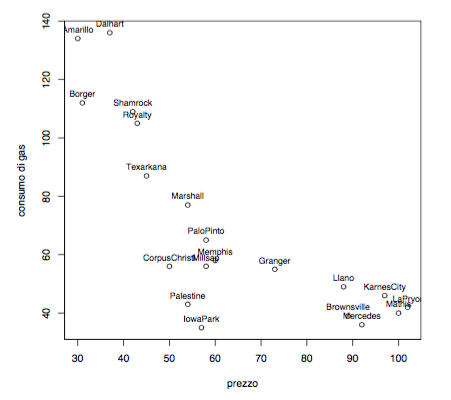
\includegraphics[width=.5\textwidth]{./notes/immagini/l7-fig1.png}
\end{figure}

\section{Un primo modello lineare}\label{un-primo-modello-lineare}

Ipotizzando che ci sia una relazione lineare è possibile utilizzare il
modello del capitolo precedente:

$$
y = \alpha + \beta x + \epsilon
$$

$$
\hat{\beta} = \frac{\cov(X,Y)}{\var(X)} \qquad \hat{\alpha} = \bar{y} - \hat{\beta}\bar{x}
$$

Utilizzando l'ambiente R si ottengono delle informazioni relative all
modello ottenuto:

\begin{verbatim}
lm(formula = gas ~ prezzo)
Residuals:
    Min      1Q  Median      3Q     Max
-40.625 -10.719  -1.136  14.073  38.292
Coefficients:
            Estimate Std. Error t value Pr(>|t|)
(Intercept)  138.561     13.552  10.225 6.34e-09 ***
prezzo        -1.104      0.202  -5.467 3.42e-05 ***
---
Signif. codes:  0 ‘***’ 0.001 ‘**’ 0.01 ‘*’ 0.05 ‘.’ 0.1 ‘ ’ 1
Residual standard error: 20.86 on 18 degrees of freedom
Multiple R-Squared: 0.6241,     Adjusted R-squared: 0.6033
F-statistic: 29.89 on 1 and 18 DF,  p-value: 3.417e-05
\end{verbatim}

Dai dati si può notare che l'indice $ R^2 $ è uguale a 0.62, il che indica un buon andamento lineare.
Inoltre come \textit{p-value} si ottiene un valore molto basso, il che porta a rifiutare l'ipotesi nulla.

Tracciando però i grafici dei residui è possibile osservare c'è una componente indipendente che non è lineare.

\begin{figure}[htbp]
	\centering
	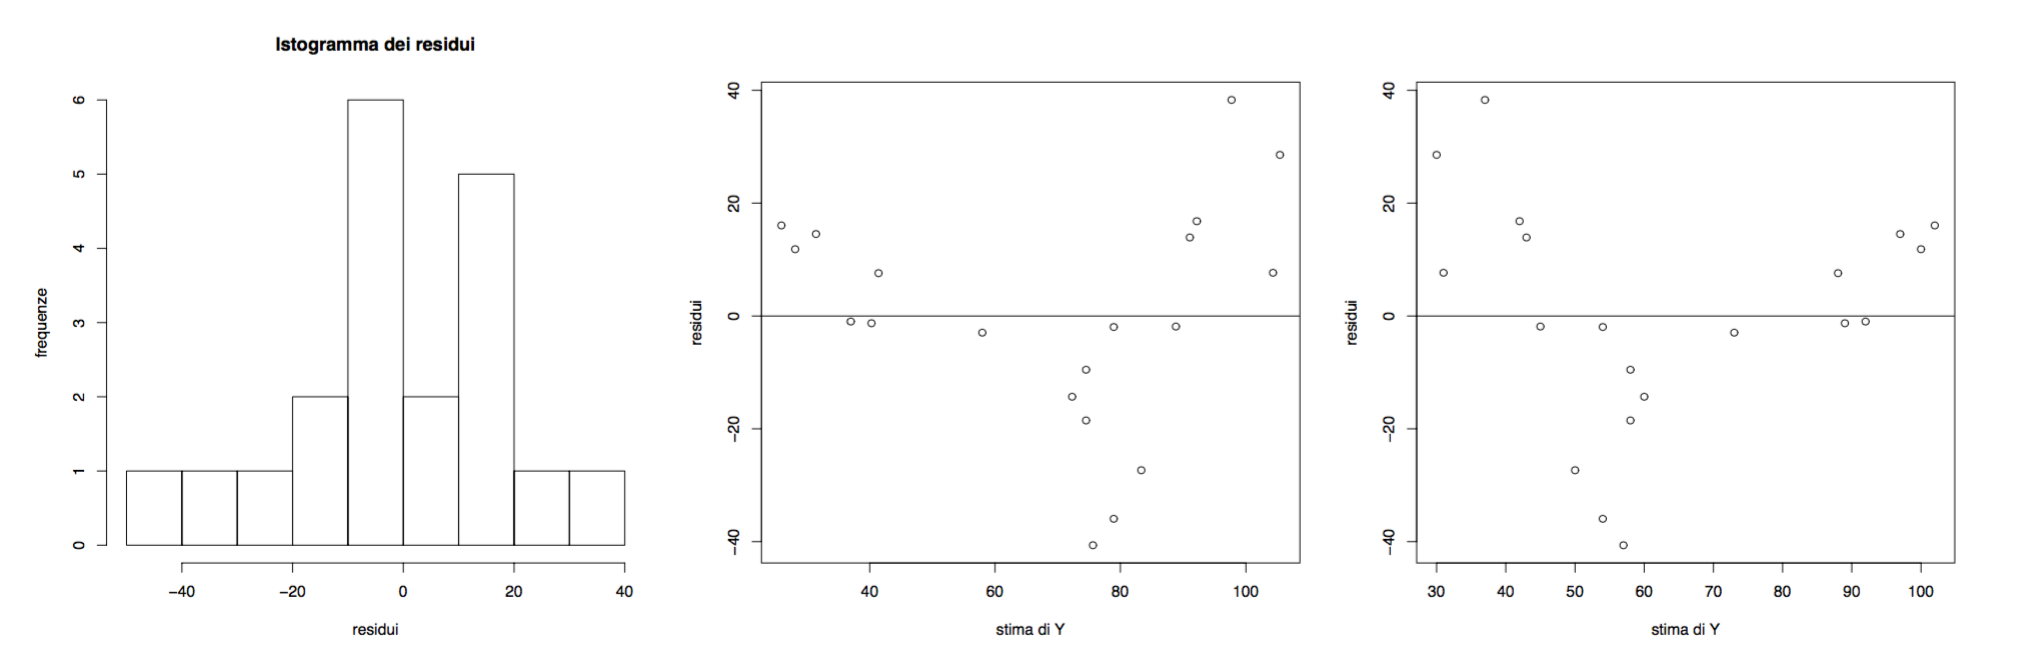
\includegraphics[width=1\textwidth]{./notes/immagini/l7-fig2.png}
	\caption{Tracciamento dei residui per il primo modello. \`{E} possibile notare la presenza di indipendente.}
\end{figure}

\section{Considerazioni sul problema e un secondo modello}\label{considerazioni-sul-problema-e-un-secondo-modello}

Considerando il problema modellato è possibile fare alcune osservazioni:

\begin{itemize}
	\item il consumatore potrebbe destinare solamente un determinato budget $ \kappa $ per l'acquisto del gas, ovvero $ x \cdot y = \kappa $.
	\item è ragionevole pensare che il consumatore debba consumare una quantità minima di gas $ \gamma $
	\item essendo il mercato del gas regolamentato, c'è un prezzo minimo di $ 7 $ centesimi al metro cubo sotto il quale non è possibile vendere il gas.
\end{itemize}

Tenendo in considerazione quanto elencato si arriva ad avere l'equazione:

$$
(x-7)(y-\gamma) = \kappa
$$

la quale può essere riscritta in un modo più simile a quella del modello lineare

$$
y = \gamma + \kappa \cdot \frac{1}{x-7}
$$

e sostituendo la variabile \textit{x} con $ z = \frac{1}{x-7} $, si ottiene proprio la stessa equazione la quale permette di calcolare la retta ai minimi quadrati.

Questo è possibile perché quello che finora è stato chiamato modello lineare è un caso particolare dei \textbf{modelli lineari nei parametri}. Ovvero la limitazione data dalla linearità non riguarda le variabili, ma riguarda solamente i \textbf{parametri} del modello.

Quando viene utilizzato il metodo dei minimi quadrati con questi modelli è necessario tenere in considerazione le trasformazioni che vengono fatte alle variabili, perché i valori calcolati ai minimi quadrati riguardano le variabili trasformate e non quelle di partenza, è necessario quindi \textbf{scalare} in modo opportuno i valori\footnote{Se viene scalata solamente la $ x $ non c'è questo problema perché i minimi quadrati considerano solamente le distanze rispetto l'asse $ y $.}.

La formulazione più generale del modello lineare è quindi

$$
g(y) = \alpha + \beta h(x) + \epsilon
$$

Il modello ottenuto per la nuova formulazione è:
\begin{verbatim}
lm(formula = gas ~ I(1/(prezzo - 7)))
Residuals:
Min    1Q  Median  3Q    Max
-29.617 -4.574 2.394 7.800 30.917
Coefficients:
Estimate Std. Error t value Pr(>|t|) 
(Intercept) 3.918 8.376 0.468 0.646
I(1/(prezzo - 7)) 3034.938 357.037 8.500 1.02e-07 *** 
---
Signif. codes: 0 ‘***’ 0.001 ‘**’ 0.01 ‘*’ 0.05 ‘.’ 0.1 ‘ ’ 1
Residual standard error: 15.19 on 18 degrees of freedom 
Multiple R-Squared: 0.8006, Adjusted R-squared: 0.7895 
F-statistic: 72.26 on 1 and 18 DF, p-value: 1.022e-07
\end{verbatim}

ovvero la retta

$$
y = 3.918 + 3034.938 \cdot \frac{1}{x-7}
$$

\begin{figure}[htbp]
	\centering
	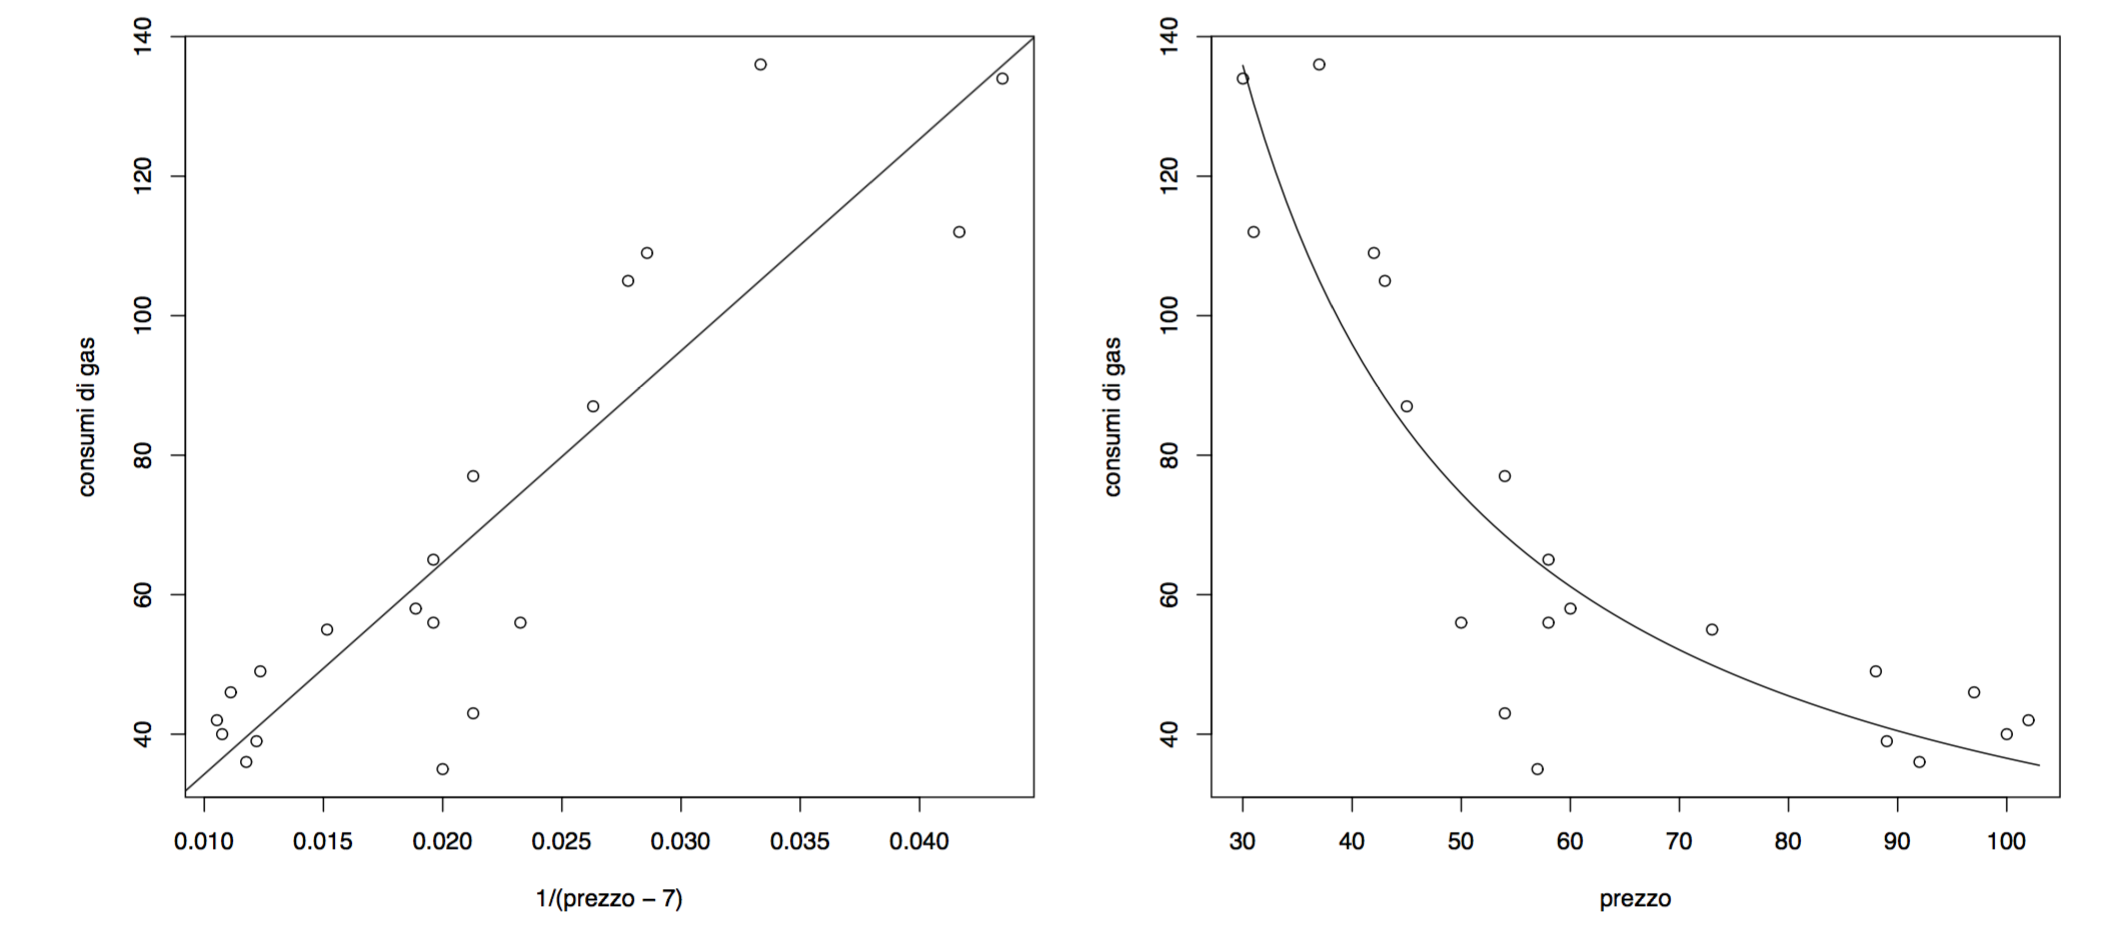
\includegraphics[width=1.1\textwidth]{./notes/immagini/l7-fig3.png}
	\caption{A destra la retta rispetto $ z $. A sinistra il modello lineare tracciato rispetto $ x $.}
\end{figure}

Dai dati del nuovo modello è possibile osservare che la varianza residua (\texttt{Residual standard error} elevato al quadrato) è passata da circa 391 a circa 207, ovvero il quadrato degli errori di previsione è stato ridotto di quasi il $ 50\% $.
Lo stesso effetto può essere visto utilizzando $ R^2 $ che da 0.6241 passa a 0.8006.

\begin{figure}[htbp]
	\centering
	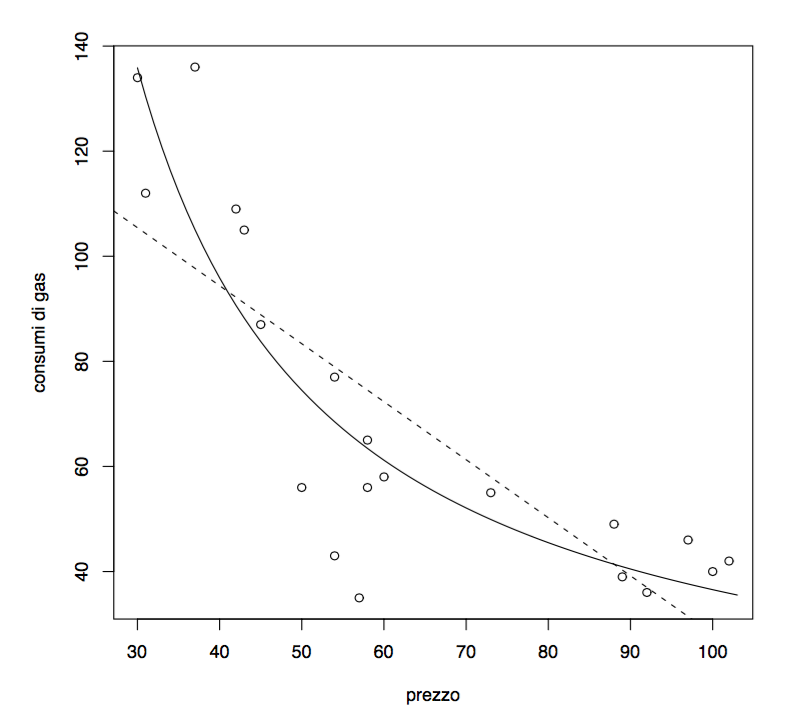
\includegraphics[width=.6\textwidth]{./notes/immagini/l7-fig4.png}
	\caption{Confronto grafico tra i due modelli.}
\end{figure}

\FloatBarrier
\section{Modello lineare con trasformate}\label{modello-lineare-con-trasformate}

\textit{Cambia il dataset di riferimento}, si vuole controllare se il reddito nazionale influisce sulla speranza di vita media dello stato. 

\begin{figure}[htbp]
	\centering
	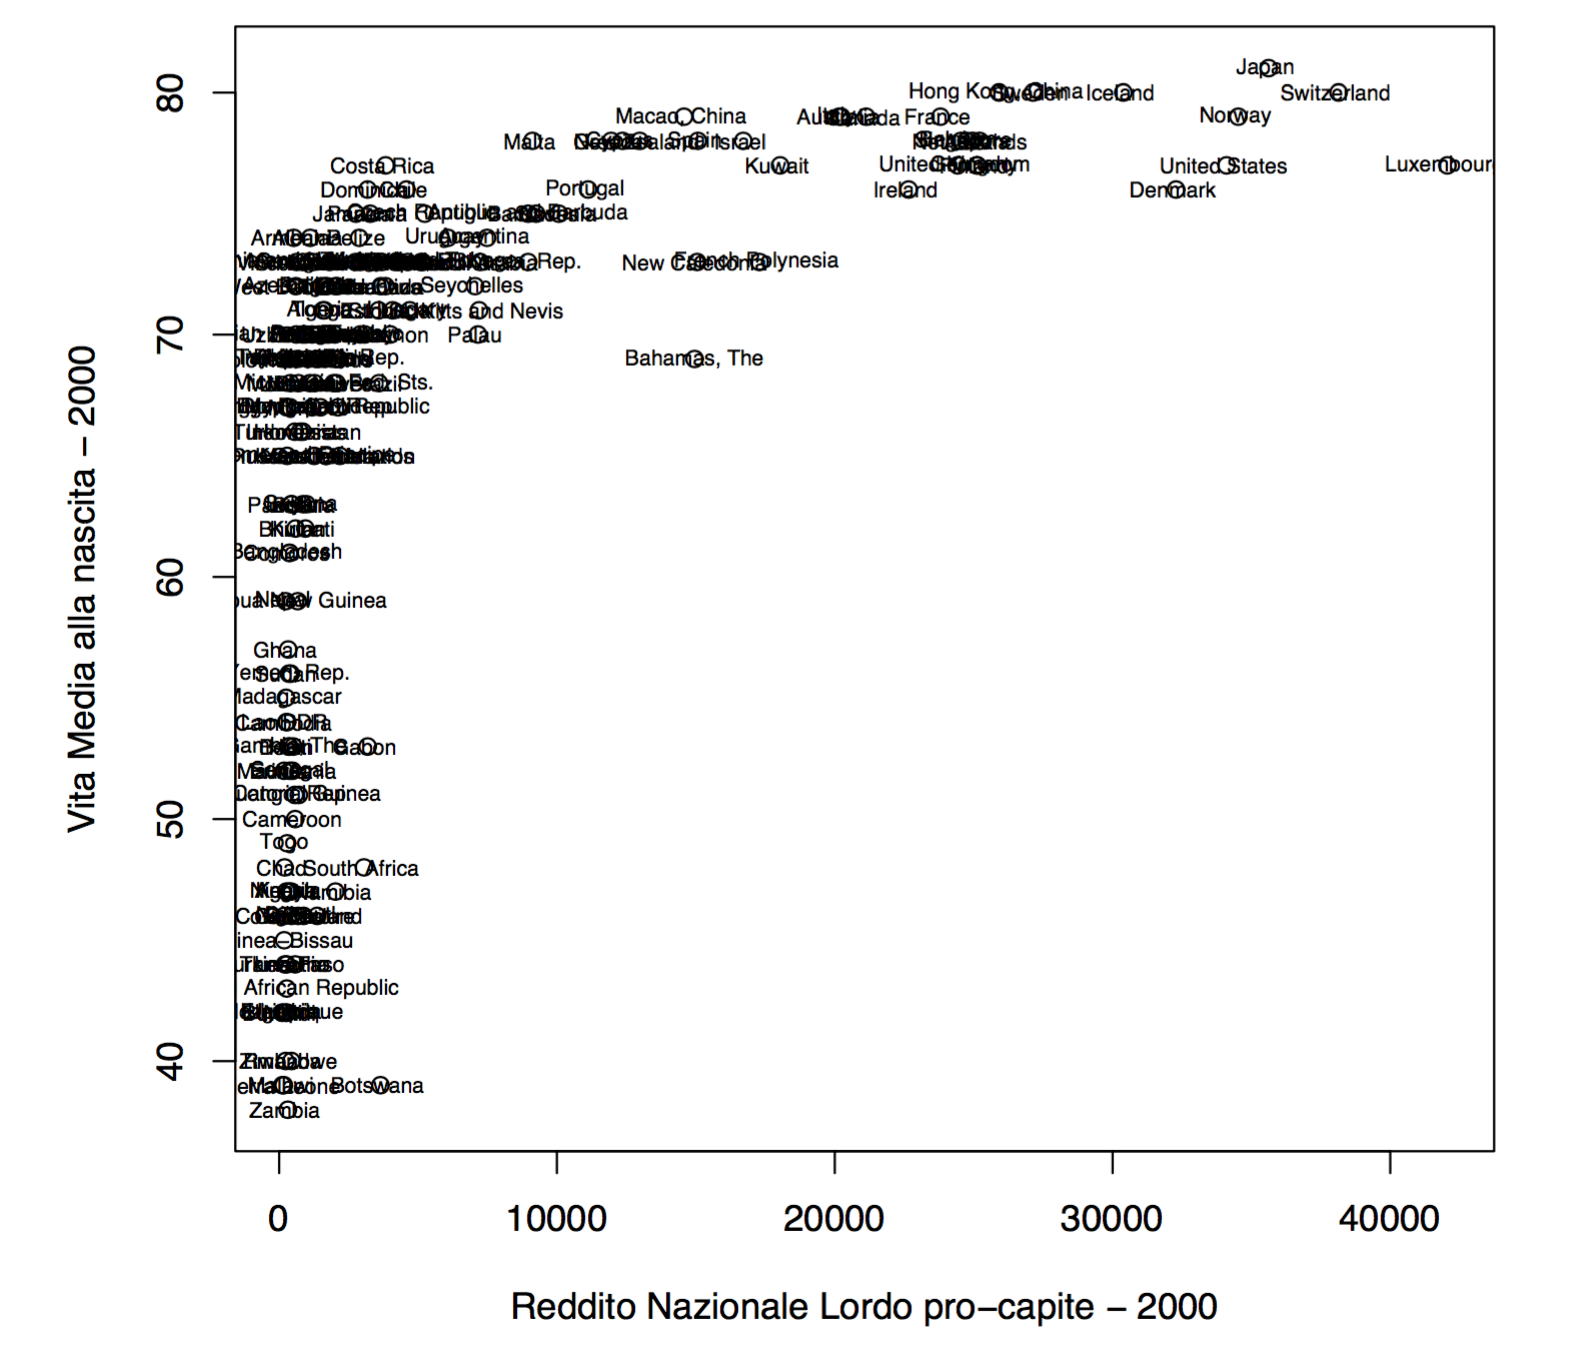
\includegraphics[width=.7\textwidth]{./notes/immagini/l7-fig5.png}
	\caption{Dataset - GNI - ELF}
\end{figure}

La prima cosa da fare è osservare come si comporta il modello lineare senza trasformazioni:

\begin{verbatim}
	lm(formula = elf ~ GNIpc)
	Residuals:
	Min    1Q  Median  3Q    Max
	-24.924 -7.512 4.119 7.431 12.948
	Coefficients:
	Estimate Std. Error t value Pr(>|t|)
	(Intercept) 6.133e+01 8.967e-01 68.390 < 2e-16 ***
	GNIpc 7.115e-04 8.230e-05 8.645 3.76e-15 ***
	---
	Signif. codes: 0 ‘***’ 0.001 ‘**’ 0.01 ‘*’ 0.05 ‘.’ 0.1 ‘ ’ 1
	Residual standard error: 9.903 on 171 degrees of freedom 
	Multiple R-Squared: 0.3041, Adjusted R-squared: 0.3 
	F-statistic: 74.73 on 1 and 171 DF, p-value: 3.757e-15
\end{verbatim}

Si può notare come l'indice $ R^2 $ sia molto basso (0.3041), ma risulta essere molto significativo perché, per il \textit{p-value} ottenuto sia ha che è improbabile che valga l'ipotesi nulla.

Tracciando il modello e il grafico dei residui è possibile notare che
\begin{itemize}
	\item La retta ottenuta non curva abbastanza e quindi non si adatta bene ai dati
	\item Il modello prevede una vita media che può essere maggiore di 90 anni, il che è abbastanza improbabile.
\end{itemize}

\begin{figure}[htbp]
	\centering
	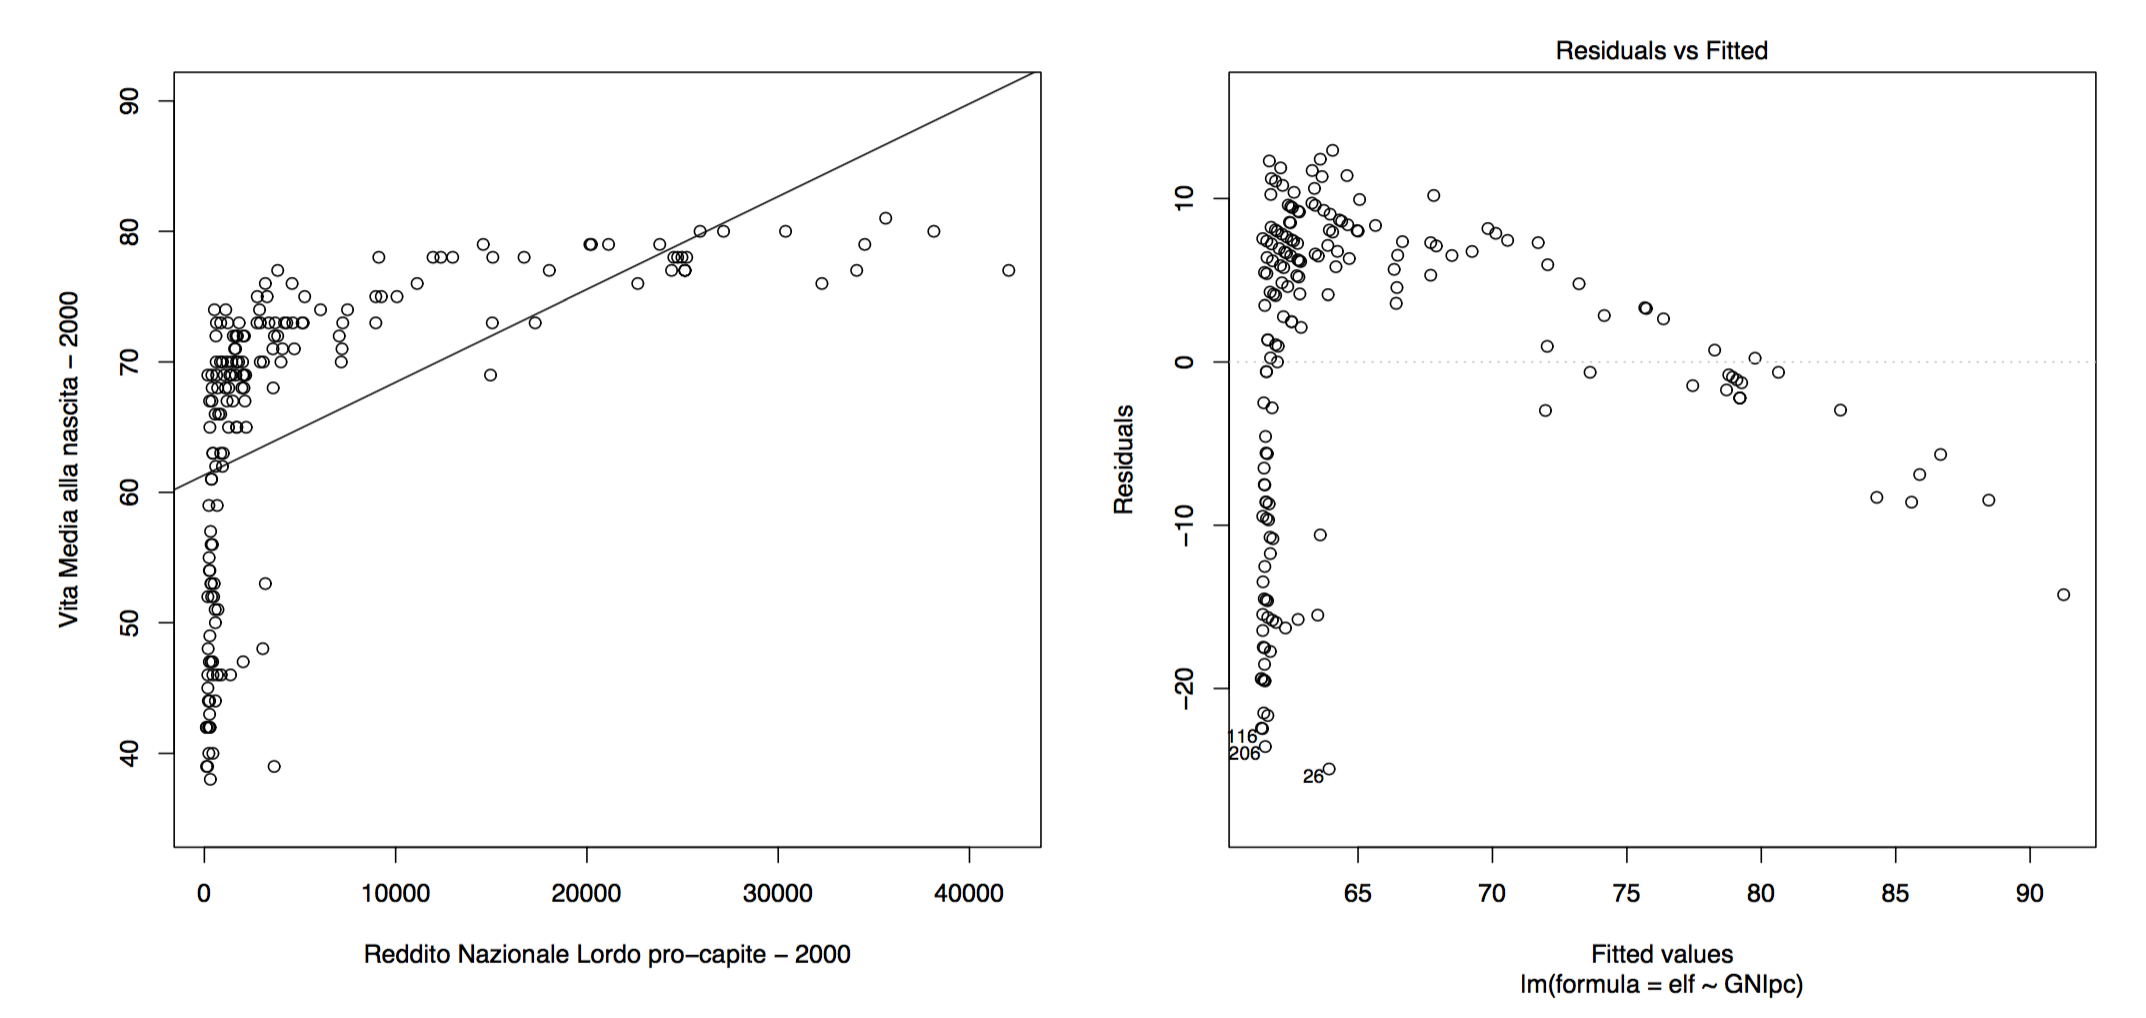
\includegraphics[width=.9\textwidth]{./notes/immagini/l7-fig6.png}
	\caption{Primo modello e residui ottenuti}
\end{figure}

Per adattare meglio la curva è possibile utilizzare la scala logaritmica per l'asse delle \textit{x}. In questo modo, al crescere del reddito viene dato via via meno peso.
Inoltre, rappresentando graficamente questa trasformazioni si ottiene una nuvola di punti più simile ad una retta.

\begin{figure}[htbp]
	\centering
	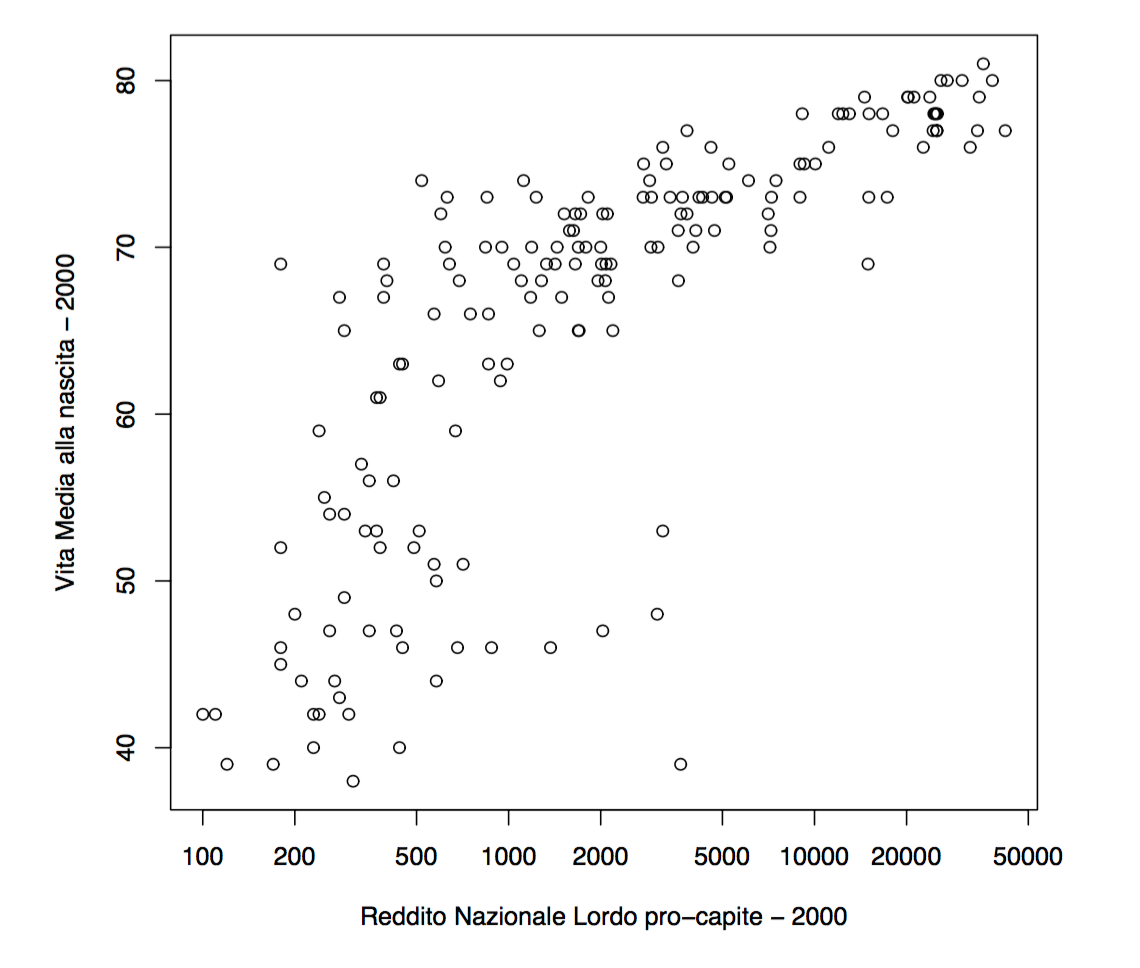
\includegraphics[width=.6\textwidth]{./notes/immagini/l7-fig7.png}
	\caption{Grafico che utilizza la scala logaritmica per i valori delle $ x $. L'asse è comunque etichettato con i valori originali.}
\end{figure}

Il modello diventa quindi

$$
(\text{vita media alla nascita}) = \alpha + \beta \log(\text{reddito nazionale pro capite})
$$

\begin{verbatim}
lm(formula = elf ~ I(logGDP), data = elf.data)
Residuals:
Min     1Q   Median   3Q     Max
-29.6591 -2.9511 0.7906 5.1050 17.4844
Coefficients:
Estimate Std. Error t value Pr(>|t|)
(Intercept) 22.6701 2.8447 7.969 2.02e-13 *** 
I(logGDP) 5.6767 0.3677 15.438 < 2e-16 ***
---
Signif. codes: 0 ‘***’ 0.001 ‘**’ 0.01 ‘*’ 0.05 ‘.’ 0.1 ‘ ’ 1
Residual standard error: 7.674 on 174 degrees of freedom 
Multiple R-Squared: 0.578, Adjusted R-squared: 0.5756 
F-statistic: 238.3 on 1 and 174 DF, p-value: < 2.2e-16
\end{verbatim}

Con questo secondo modello si ottiene un indice $ R^2 $ doppio rispetto al precedente e questo può essere osservato anche nella rappresentazione grafica del nuovo modello.

\begin{figure}[htbp]
	\centering
	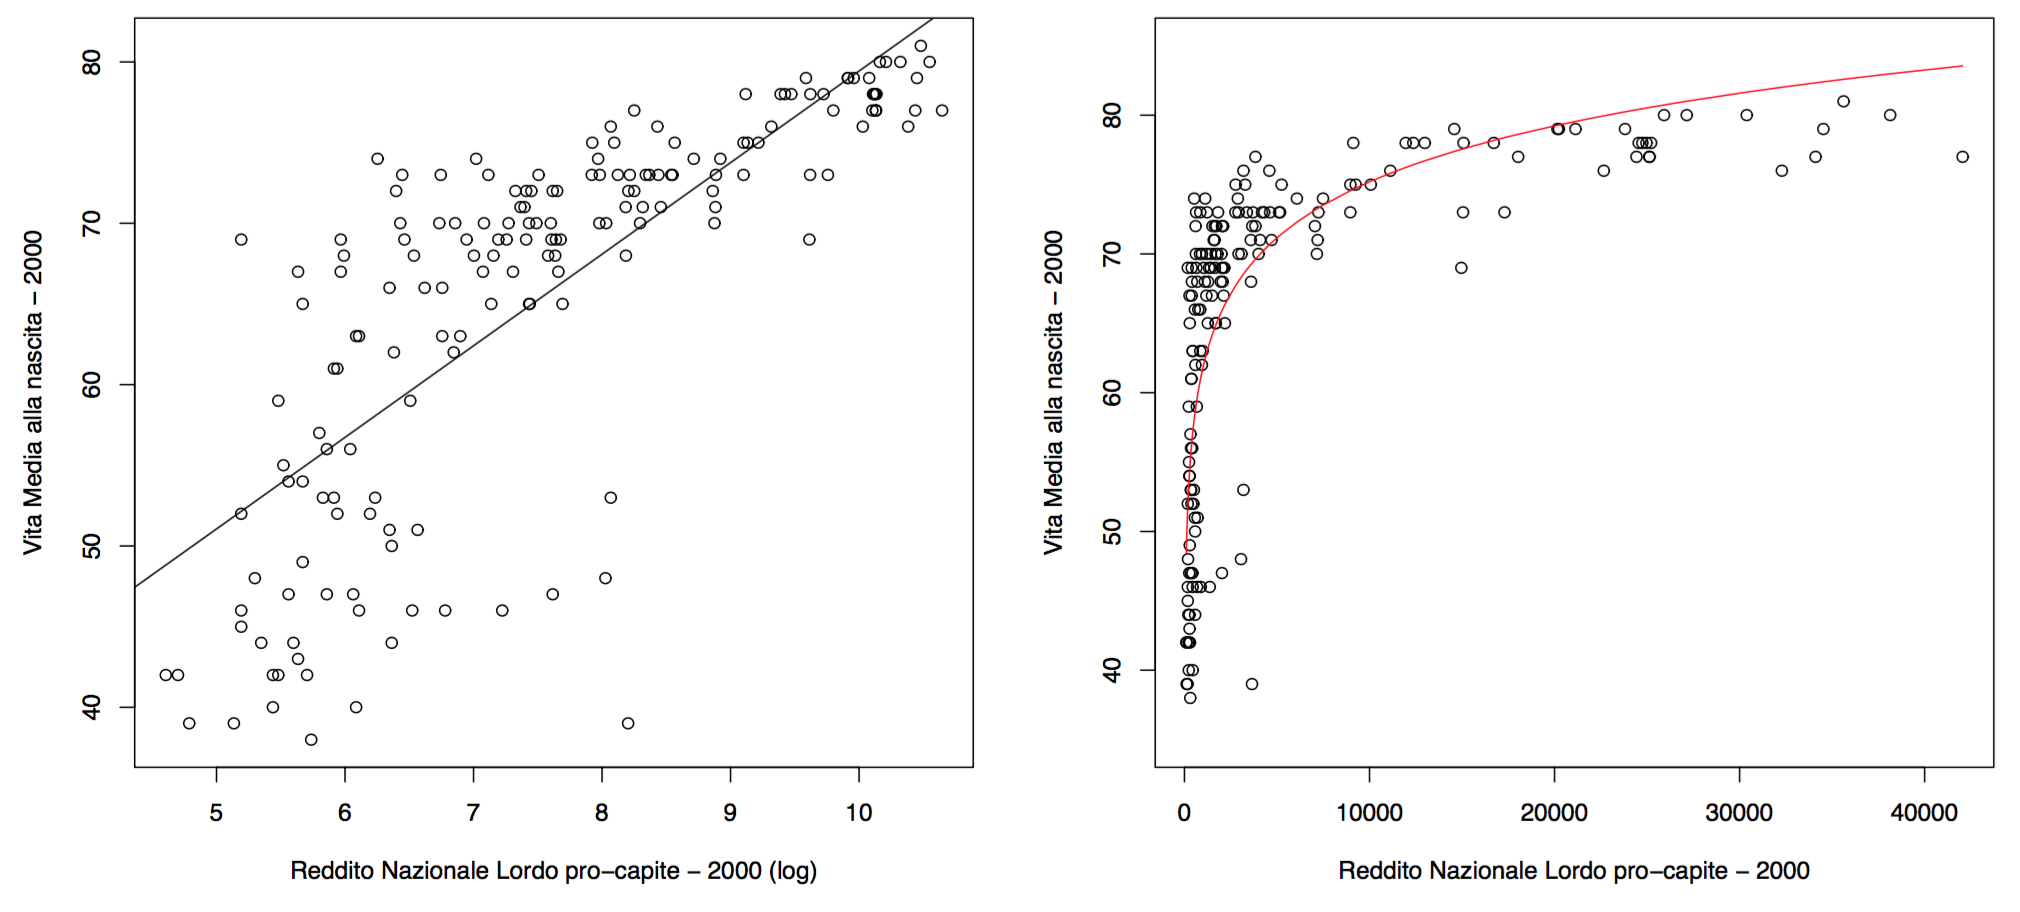
\includegraphics[width=.9\textwidth]{./notes/immagini/l7-fig8.png}
	\caption{Secondo modello: a sinistra con la scala logaritmica, a destra normale.}
\end{figure}

C'è però ancora un problema che riguarda i valori estremi che non vengono approssimati bene dalla curva e lo si può notare anche dai residui.

\begin{figure}[htbp]
	\centering
	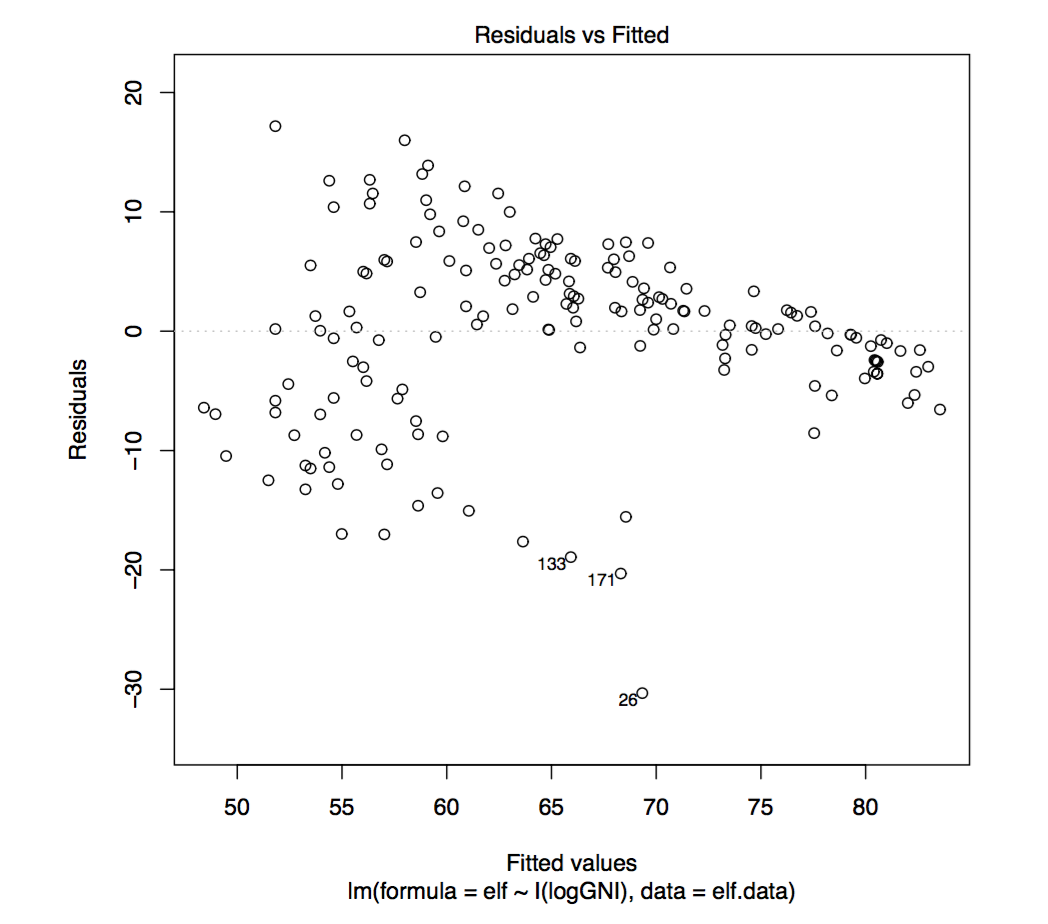
\includegraphics[width=.6\textwidth]{./notes/immagini/l7-fig9.png}
	\caption{Residui per il secondo modello }
\end{figure}

Un'ulteriore modifica può essere quella di trasformare anche la variabile risposta, elevandola alla quinta, in modo da dare maggior peso ai valori maggiori.

Il modello ottenuto è quindi dato da

$$
(\text{vita media alla nascita})^5 = \alpha + \beta \log(\text{reddito nazionale pro capite}) + \epsilon
$$

Da notare che con questa formulazione le ipotesi sugli errori (media nulla, varianza costante, distribuzione normale, ecc.) \textbf{devono valere per gli errori su scala trasformata}.

Una volta calcolato il modello si ottiene

\begin{verbatim}
lm(formula = elf.5 ~ logGNI, data = elf.data)
Residuals:
Min        1Q        Median    3Q       Max
-1.801e+09 -2.817e+08 7.965e+06 3.036e+08 1.334e+09
Coefficients:
Estimate Std. Error t value Pr(>|t|) 
(Intercept) -2.345e+09 1.832e+08 -12.80 <2e-16 *** 
logGNI 5.164e+08 2.376e+07 21.73 <2e-16 ***
---
Signif. codes: 0 ‘***’ 0.001 ‘**’ 0.01 ‘*’ 0.05 ‘.’ 0.1 ‘ ’ 1
Residual standard error: 4.89e+08 on 171 degrees of freedom 
Multiple R-Squared: 0.7341, Adjusted R-squared: 0.7326 
F-statistic: 472.2 on 1 and 171 DF, p-value: < 2.2e-16
\end{verbatim}

\begin{figure}[htbp]
	\centering
	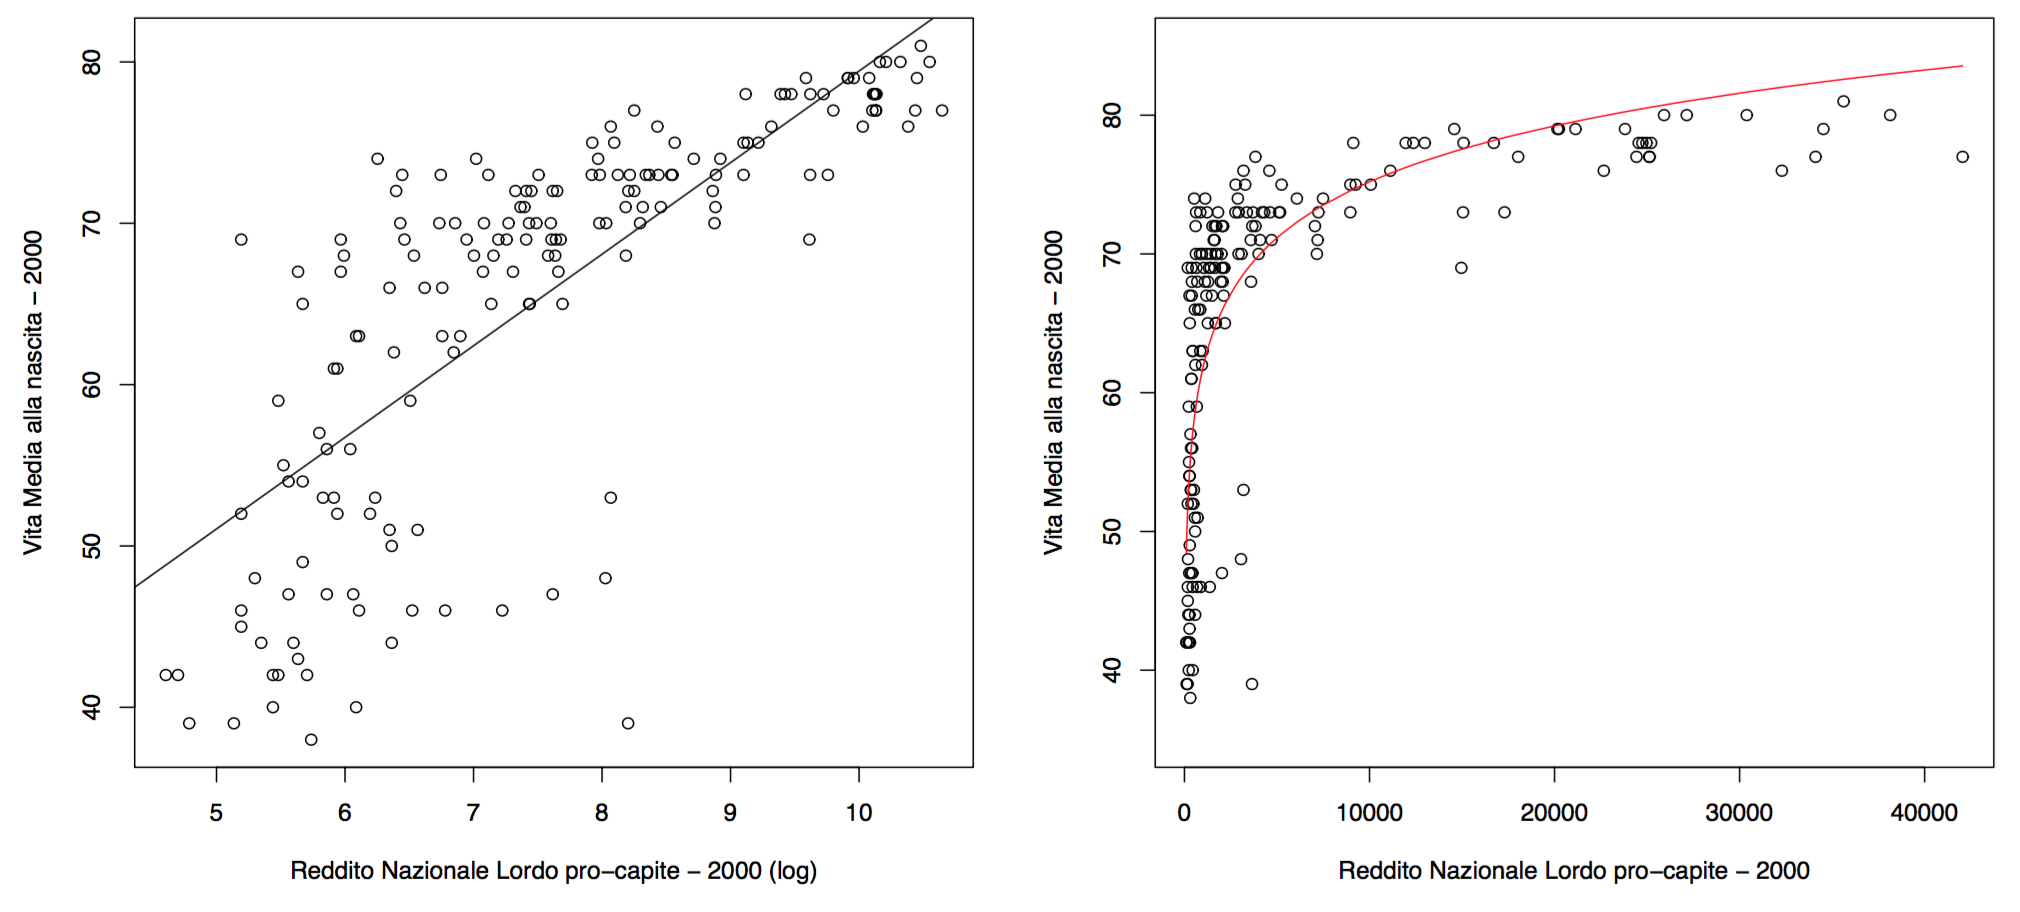
\includegraphics[width=.9\textwidth]{./notes/immagini/l7-fig8.png}
	\caption{Terzo modello: a sinistra con la scala originale e a destra i residui.}
\end{figure}

L'indice $ R^2 $ ottenuto fa riferimento ai residui calcolati sulla scala trasformata, quindi per avere un'indice di adattamento dei dati è possibile utilizzare la media dei quadrati dei residui per la variabile originale:

$$
\frac{1}{n}\sum\limits_{i=1}^n \bigg[ \big(\text{vita media alla nascita}\big)_i - \sqrt[5]{\big(\alpha + \beta \log(\text{reddito nazionale pro capite})_i\big)}\bigg]^2
$$

Calcolando questo valore si ottiene 55.08, mentre con il secondo modello si aveva la varianza dei residui pari a 58.89. Si ottiene quindi una riduzione del $ 6\% $ del quadrato degli errori di previsione.









